%!TEX root = ../thesis.tex
%Adding the above line, with the name of your base .tex file (in this case "thesis.tex") will allow you to compile the whole thesis even when working inside one of the chapter tex files


\chapter{Introduction to Radio Interferometry} 
\label{chap:2}

The poor spatial resolution provided by a single dish radio antenna can cause difficulties in obtaining accurate flux density measurements of radio astronomical sources, especially at long wavelengths. A single dish radio antenna is unable to distinguish against background radio emitters located in the primary beam, and therefore the the observed flux density can contain emission from unrelated sources. This limitation can be overcome through interferometry. An interferometer acts as a spatial filter, and can discriminate against smooth backgrounds while its higher resolution allows seperation of the target from nearby confusing sources. 

\section{Radio Antenna Basics}\label{sec:1}
The quality and properties of the final radio image produced from a synthesis array are partially dependent on the properties of the the individual antennae in the array. The most important such properties are discussed in the following sections and include aperture size, aperture efficiency, pointing accuracy, sidelobe level and noise temperature. We define the radio antenna as the piece of equipment which converts the electromagnetic waves emitted from the observed source into an electric current ready to be input into to the first low noise amplifier where the signal is at the radio/sky frequency, $\nu _{\rm{RF}}$.
\subsection{Radio Antenna Formulae}\label{subsec:1}
The power gain of a transmitting antenna is a measure of the antenna's capability of converting power into radio waves in a specific direction. In radio astronomy, the receiving counterpart of transmitting power gain is the effective collecting area of an antenna, $A$($\nu$,$\theta$,$\phi$), where $\nu$ is frequency and $\theta$ and $\phi$ are direction coordinates. An ideal radio antenna would collect all incident radiation from a distant point source and convert it to electrical power. The total spectral power $P_{\nu}$, collected by it would then be a product of its geometric area and the incident spectral power per area, or flux density $F_{\nu}$. By analogy then, the effective area of a real radio antenna is defined
\begin{equation}
A(\nu,\theta,\phi)= \frac{P_{\nu}}{F_{\nu}}=\frac{P}{I(\nu,\theta,\phi)\Delta \nu \Delta \Omega}
\end{equation}
where $I$($\nu$,$\theta$,$\phi$) is the source brightness in units W m$^{-2}$ Hz$^{-1}$ sr$^{-1}$ that the antenna is pointing at and $P$ is the power (in Watts) received by the antenna in bandwidth $\Delta \nu$ from element $\Delta\Omega$ of solid angle. The normalized antenna reception pattern $\mathcal{A}$, often referred to as the power pattern due to the duality between receiving and transmitting, is defined as 
\begin{equation}
\mathcal{A}(\nu,\theta,\phi)= \frac{A(\nu,\theta,\phi)}{A_{0}}
\end{equation}
where $A_0$ (m$^2$) is often referred to as the effective area of the antenna and is the response at the center of the main lobe of $A$($\nu$,$\theta$,$\phi$) [i.e. A($\nu$,0,0)]. Then the beam solid angle, $\Omega _{A}$, of the primary beam is 
\begin{equation}
\Omega _{A} = \int \!\!\! \int _{\rm{all\ sky}} \mathcal{A}(\theta,\phi) d \Omega
\end{equation}
and is a measure of the field of view of the antenna. 

In the case of an isotropic antenna [i.e., $\mathcal{A}(\nu,\theta,\phi)=1$], it can be shown that the product of the effective area and the primary beam solid angle is equal to the square of the wavelength \citep{kraus_1986}
\begin{equation}
A_{0}\Omega _{A} = \lambda ^2.
\label{eq:kraus}
\end{equation}
$\Omega _{\rm{A}}$ has its maximum possible value of $4\pi$ if $\mathcal{A}$ is everywhere equal to 1. This means that the primary antenna can see the whole sky with equal sensitivity. Even though a large field of view is usually desirable in radio astronomy, Equation \ref{eq:kraus} ensures that for any given wavelength, when $\Omega _{A}$ is a maximum, the power received is a minimum and therefore the sensitivity is also at a minimum. To improve sensitivity, one could increase the collecting area of the antenna, but Equation \ref{eq:kraus} then ensures that the field of view must decrease. Thus, when deciding on the primary antenna size in a synthesis array, there is always a trade-off between field of view and sensitivity. 

In reality, an antenna cannot radiate isotroptically and will radiate preferentially in one or more directions. A Fourier transform relationship exists between the complex voltage distribution of the field, $f(u,v)$, in the aperture of the antenna and the complex far-field voltage radiation pattern, $F(l,m)$, of the antenna \citep{kraus_1986}
\begin{equation}
F(l,m)=\int\!\!\! \int _{\rm{aperture}} f(u,v)e^{2\pi i(ul+vm)}dudv
\end{equation}
and
\begin{equation}
f(u,v)=\int ^{\infty} _{\infty}\int ^{\infty} _{\infty} F(l,m)e^{-2\pi i(ul+vm)}dldm
\label{eq:illum1}
\end{equation}
where
\begin{equation}
u=\rm{sin}\theta \rm{cos}\phi \ \  \rm{and} \ \ \mathit{v}=\rm{sin}\theta \rm{sin}\phi
\label{eq:illum2}
\end{equation}

\begin{figure}[hbt!]
\centering 
\mbox{
          \includegraphics[trim=60pt 10pt 80pt 30pt,clip,width=7.0cm]{/home/eamon/thesis/figures/antenna_beam/fig2a.ps}
          \includegraphics[trim=60pt 10pt 80pt 30pt,clip,width=7.0cm]{/home/eamon/thesis/figures/antenna_beam/fig2b.ps}
          }
\mbox{
          \includegraphics[angle=90,trim= 10pt 80pt 30pt 60pt,clip,width=8.0cm]{/home/eamon/thesis/figures/antenna_beam/fig2c.ps}
          }
\caption[Radiation and power pattern of a uniformly illuminated antenna.]{\textit{Top Left:} A uniformly illuminated 1-D aperture $f(u)$. \textit{Top Right:} The Fourrier transform of $f(u)$ gives the antenna radiation pattern in the far-field, $F(l)$. \textit{Bottom:} The power pattern of the antenna is given by $\mathcal{A}=|F(l)|^2$.}
\label{fig2a}
\end{figure}

are the antenna coordinates and $l$ and $m$ are their Fourrier counterparts. The from of $f(u,v)$ is determined by the manner in which the antenna feed illuminates the aperture. Therefore Equations \ref{eq:illum1} and \ref{eq:illum2} tell us that the radiation pattern in the far-field of a two-dimensional aperture is the two-dimensional Fourier transform of the aperture field illumination. For a uniformly illuminated 1-D aperture shown in Figure \ref{fig2a}, the radiation pattern in the far-field is the \textit{sinc} function. The radiation pattern in the far-field, $F(l,m)$, of such an antenna is related to the antenna power pattern, $\mathcal{A}$, by $\mathcal{A}=|F(l,m)|^2$. This power pattern is known as the Airy pattern if the antenna is uniformly illuminated and is also shown in Figure x. The central peak of this power pattern is called the main beam while the smaller secondary peaks are called sidelobes. The antenna is maximally sensitive to radiation from the direction of the peak of the beam, but is also slightly sensitive to radiation in the direction of the side lobes. The half-power beamwidth (HPBW) of the main beam, $\theta_{\rm{HPBW}}$, is a term commonly used in the literature to describe the field of view of an antenna/interferometer and satisfies 
\begin{equation}
\theta_{\rm{HPBW}} \propto \frac{\lambda}{D}
\end{equation}
where $D$ is the diameter of the antenna. The constant of proportionality varies slightly with the illumination taper and can be shown to be equal to $\sim 0.89$ for a uniformly illuminated linear aperture and $\sim 1.2$ for a Gaussian illuminated aperture. When the sky is scanned with a single antenna, then this HPBW is the resolution of the resulting map. 

\subsection{Antenna Structural Design}\label{subsec:2}
The design of the primary antenna element of an interferometric array will depend on the wavelength range to be observed. In general, wire antennas are used for wavelengths longer than $\sim 1$ m, while reflector antennas are typically used at shorter wavelengths. The reason why the more simple and less expensive wire antennas are not used at all wavelengths is given by Equation \ref{eq:kraus}. For an isotropic antenna, this equation tells us that the effective area is just
\begin{equation}
A_{0} = \frac{\lambda ^2}{4\pi}.
\end{equation}
Therefore, at short wavelengths a non-directional antenna such as a dipole, will have a small effective collecting area, giving it poor sensitivity for reception. Thus, wire antennas can be used at long wavelengths as they have sufficient collecting area, but cannot be used at shorter wavelengths as an impractical amount would be needed to produce useful collecting areas. Since the interferometric arrays used in this thesis use reflector antennas, the rest of this section will focus on them.\\
\\
\textit{Choice of Antenna Mount.} Nearly all interferometric arrays consist of antennas which have altitude over azimuth (altazimuth) mounts. These antennas lie on a horizontal azimuth track on which the antenna can turn in azimuth, and a horizontal elevation axle about which the antenna changes in zenith angle. The main advantage of such a design is simplicity and thus lower cost. Gravity always acts on the reflector in the same plan thus reducing the problem of keeping the reflector profile accurate during the duration an observation. However, sources close to the zenith cannot be observed due to the high rate of azimuth rotation required. Also, the beam rotates with respect to the source for long duration observations which can affect the dynamic range of total intensity images of very large sources. The other type of mount occasionally used is the equatorial mount. Its polar axis is aligned parallel to the axis of rotation of the Earth and therefore only needs to rotate about the declination axis to observe a source. Its beam also doesn't have the beam rotation problem encountered by the altazimuth design and can track sources close to the zenith. Its major disadvantage and the reason for its scarce usage is the complexity of its design and resulting increased cost. \\
\\
\textit{Choice of Antenna Optics.} In Figure \ref{fig2d} we show the main optical systems which can be used to feed a large radio reflector. The prime focus system (e.g. used in the Giant Meter Radio Telescope) has the advantage that it can be used at long wavelengths where the use of secondary focus feeds (i.e. sub-reflectors) become impractical. However, access to, and space for, the feed and receiver is limited and sensitivity can be lost due to spillover noise from the ground. The other designs have the advantage of easier access to the feeds and receivers and less spillover noise from the ground. The off-axis Cassegrain (e.g. used in the Very Large Array) has also the advantage of increased frequency capability as many feeds can be located in a circle around the centre of the reflector and a slight rotation of the sub-reflector is all that is required to change observing frequency. The receivers and feeds in the Naysmith geometry (e.g used in the Combined Array for Research in Millimeter wave Astronomy) are located externally to the antenna structure. Finally, the offset Cassegrain (e.g. used in the Green Bank Telescope) has no blockage and will have a circularly symmetric beam with low sidelobes but the increase complexity of its structure leads to increased costs. 

\begin{figure}[hbt!]
\centering 
          \includegraphics[trim=10pt 40pt 60pt 50pt,clip,width=10.0cm,angle=-90]{/home/eamon/thesis/figures/fig2d.ps}
\caption[Common optical systems used for radio antennas.]{(\textit{a}) Prime focus, (\textit{b}) Naysmith, (\textit{c}) Off-axis Cassegrain, (\textit{d}) Offset Cassegrain (Figure adapted from \cite{taylor_1999}).}
\label{fig2d}
\end{figure}

\subsection{Antenna Performance Parameters}\label{subsec:3}
\textit{Aperture Efficiency.} The geometric collecting area of a parabolic antenna, $A_{\rm{geo}}$ ($=\pi D^2/4$), is related to the effective area (i.e. the collecting area when pointing directly at a source) via the dimensionless quantity, $\eta$, known as the aperature efficiency where
\begin{equation}
\eta = \frac{A_0}{A_{\rm{geo}}} 
\end{equation}
and is always less than unity. The aperture efficiency directly impacts on the sensitivity of the interferometric array and can be defined as the product of a number of different efficiency loss factors, 
\begin{equation}
\eta = \eta _{\rm{sf}}\eta _{\rm{bl}}\eta _{\rm{s}}\eta _{\rm{t}}\eta _{\rm{misc}}.
\end{equation}
The surface efficiency, $\eta _{\rm{sf}}$, accounts for the aperture efficiency loss as a result of reflector profile inaccuracies. Such inaccuracies result in the electric field from various parts of the aperture not adding together in phase at the feed leading to a decrease in power. The aperture blockage efficiency, $\eta _{\rm{bl}}$, accounts for the fact that the subreflector (or feed) and its support structure result in a reduction in the incident radiation on the antenna. The feed spillover efficiency, $\eta _{\rm{bl}}$, is best understood if the antenna is considered in transmission rather than in reception mode, and  is defined as the fraction of power radiated by the feed that is intercepted by the reflector for a prime focus system, or by the subreflector for a Cassigrain system. The illumination taper efficiency, $\eta _{\rm{t}}$, accounts for the fact that the feed pattern does not illuminate the primary reflector uniformly but illuminates the outer part of the reflector at a lower level than the inner part. Finally, the miscellaneous efficiency losses such as reflector diffraction and feed position phase errors are accounted for in $\eta _{\rm{misc}}$.
\\
\\
\textit{Pointing Accuracy.}
The main lobe of an antenna's power pattern will usually not point exactly in the desired direction due to gravity deformations, wind pressure deformations, and mechanical inaccuracy. The angular offset, $\Delta \theta$, between the actual and desired pointing direction is called the pointing error. Usually, the desirable pointing error of  an antenna at the highest operational frequency is $\Delta \theta < \theta _{\rm{HPBW}}/20$ \citep{taylor_1999}. With this specification reached, an antenna pointing at a compact source will suffer negligible intensity variations as $\mathcal{A}(\theta _{\rm{HPBW}}/20) > 0.99$. However, this pointing error of only $\theta _{\rm{HPBW}}/20$ will still have a substantial effect on the accuracy of the outer image. For example, a source located at the half power point will suffer a substantial fractional intensity variation of $2\mathcal{A}(\theta _{\rm{HPBW}}/2+\theta _{\rm{HPBW}}/20) \simeq 0.86$. The blind pointing of a VLA antenna is only about 10$^{\prime\prime}$ and can be much worst in daytime, occasionally exceeding 1$^{\prime}$. This means that at Q-band (45 GHz; 0.7 cm), which is the highest observing frequency on the VLA, the pointing error is only at best $\theta _{\rm{HPBW}}/6$, and at worst $>\theta _{\rm{HPBW}}$, meaning that the target may lie outside of the primary beam. To overcome this problem of large antenna pointing errors at high frequencies with the VLA, a technique known as referenced pointing is implemented. This technique will be discussed in detail in Chaper 3. 

\section{The Antenna Backend}\label{sec:2}

\section{Fundamentals of Radio Interferometry}\label{sec:3}
The angular resolution $\Delta \theta$ of a radio antenna is the minimum angular separation which two point sources can have in order to be recognized as separate objects. The \textit{Rayleigh criterion} is the generally accepted criterion for defining the angular resolution of a filled circular aperture of diameter $D$, at the observational wavelength $\lambda$ and is given as
\begin{equation}
\Delta \theta=1.22\frac{\lambda}{D} \ \ \rm{rad}.
\label{eq:rayleigh}
\end{equation}
The Rayleigh criterion states that two objects are resolved when the first null of the diffraction pattern of one object coincides with the maximum of the diffraction pattern of the other. An immediate consequence of Equation \ref{eq:rayleigh} is that at large wavelengths, the angular resolution becomes large unless the diameter of the aperture can be increased substantially. In order to achieve modest angular resolution at radio wavelengths with a single radio antenna then, the diameter becomes impractically large. For example, in order to achieve an angular resolution of 1$^{\prime \prime}$ at 6 cm a 12 km aperture would be required. Radio interferometry is a technique used in radio astronomy to overcome this problem of poor resolution at long wavelengths. 

\subsection{Young's Slits}\label{subsec:4}
The basic principles of interferometry can be understood through Young's double-slit experiment. If coherent radiation emitted from a distant point source propagates through two slits, an illumination pattern composed of bright and dark fringes is observed. The phenomenon is a result of the constructive and destructive interference between the secondary waves produced by the slits. The fringe separation is $\lambda /B$, where $B$ is the projected separation of the slits and is called the baseline. The fringe contrast which is historically known as the fringe visibility, $V$, can be written as
\begin{equation}
|V| = \frac{I_{\rm{max}}-I_{\rm{min}}}{I_{\rm{max}} + I_{\rm{min}}}
\end{equation}
where $I_{\rm{max}}$ and $I_{\rm{min}}$ are the maximum and minimum intensity of the fringes, respectively. In other words, the fringe visibility is the fringe amplitude normalized by the sum of the maximum and minimum intensity.
In the simple case shown in Figure \ref{fig2e}a, the angular size of the source is  $\ll \lambda/B$ and the fringe visibility is 1. In interferometry, this equates to the situation in which the source size is smaller than the synthesized beam and only an upper limit of the source size can be obtained.

\begin{figure}[hbt!]
\centering 
          \includegraphics[trim=0pt 0pt 0pt 0pt,clip,width=12.0cm]{/home/eamon/thesis/figures/youngs.ps}
\caption[Common optical systems used for radio antennas.]{The resulting fringe pattern produced by Young's slits under various situations. The source is shown on the left side of the slits in each panel, while the separate fringe patterns (colors) along with the added fringe pattern (black) is shown on the right of the slits. (\textit{a}) Point source at infinity, (Visibility = 1). Finges are seperated by an angular distance of $\lambda /B$. (\textit{b}) An increase in source size results in a drop in visibility. (\textit{c}) When the source size is equal to $\lambda /B$, the visibility is zero. (\textit{d}) If the source size remains the same as in (c) and the slit spacing is reduced, then the fringes re-appear. (Figure adapted from \cite{jackson_2008}).}
\label{fig2e}
\end{figure}

In Figure \ref{fig2e}b, the angular size of the source is now larger and can be thought of as a sequence of point sources each emitting radiation which is uncorrelated with the emission from the others. An angular shift of $\phi$, in the sources position results in a shift in the corresponding fringe pattern by the same angle the other way. The total interference intensity pattern is then just the sum of these individual patterns and the visibility is reduced. When the extension of the source equals $\lambda/B$, the fringes disappear and give a constant illumination pattern. In this case the fringe visibility is zero and the source is completely resolved.
\subsection{The Two-element Interferometer}\label{subsec:5}
Essential Radio 
\section{Synthesis Imaging}\label{sec:4}
Essential Radio 